Given the size of the tree to be explored (at least 400 million nodes), a Root parallelisation strategy on computers could not be applied. A 11 million nodes tree require about 2 Go of RAM\ref{fig:RAMTree}. Should it be timed by 40 and the number of core, there would be not enough RAM.
\begin{figure}[H]
\centerline{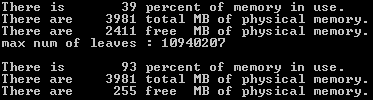
\includegraphics[width=0.6\textwidth]{Parallelisation/Computer/Img/RAM.png}}
\caption{\label{fig:RAMTree}\textit{Memory used before and after the creation of nodes}.}
\end{figure}

A tree parallelisation strategy has to be implemented on the computer. It can be done by multithreading the \textit{While // loop simulations} descriped in the base algorithm implementation\ref{fig:MCTSAlgorithm}.

Using OpenMP, this is easily implented with a single \#pragma statement :\\
\textbf{\#pragma omp parallel shared(i,timeend)}\\
where \textit{i}, the number of simulation run and \textit{timeend}, the time until simulations are to be run are defined as shared variables.

In order to prevent any conflict between threads, a small critical section has to control the tree expansion. This can be done by using the following statement before the call of \textit{UpdateNode(node)}:\\
\textbf{\#pragma omp critical}